\begin{minipage}{0.75\linewidth}
\begin{figure}[h]
    \centering
    \begin{adjustbox}{max width=1.0\linewidth, keepaspectratio}
        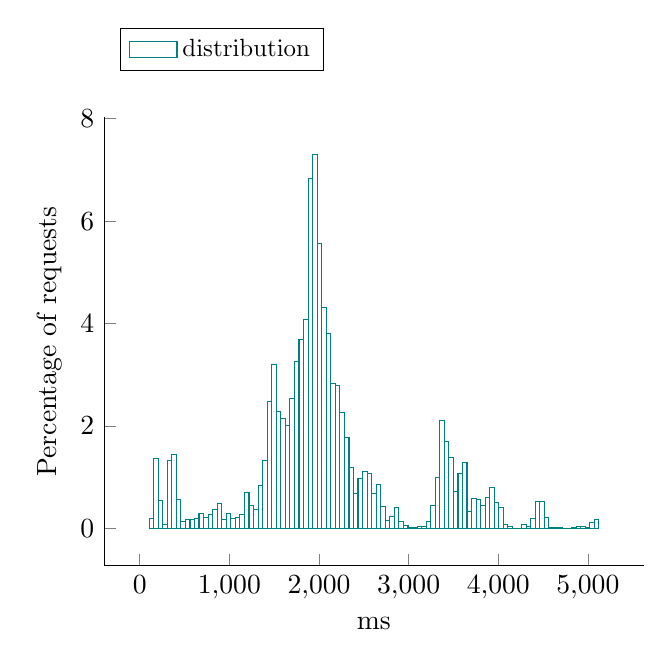
\begin{tikzpicture}
            \begin{axis}[ylabel = Percentage of requests, 
xlabel = ms, 
legend style = {nodes={scale=0.9, transform shape}, at={(0.03,1.2)}, anchor=north west, draw=black, fill=white, align=left, legend columns=3},
area style, mark size = 0pt,
 cycle list name = exotic,
  axis lines* = left]
		\addplot +[ybar interval] coordinates {
			 (104, 0.1875)
			 (154.68, 1.35938)
			 (205.36, 0.546875)
			 (256.04, 0.078125)
			 (306.72, 1.32812)
			 (357.4, 1.4375)
			 (408.08, 0.5625)
			 (458.76, 0.125)
			 (509.44, 0.171875)
			 (560.12, 0.171875)
			 (610.8, 0.1875)
			 (661.48, 0.296875)
			 (712.16, 0.203125)
			 (762.84, 0.265625)
			 (813.52, 0.359375)
			 (864.2, 0.484375)
			 (914.88, 0.171875)
			 (965.56, 0.296875)
			 (1016.24, 0.1875)
			 (1066.92, 0.21875)
			 (1117.6, 0.265625)
			 (1168.28, 0.703125)
			 (1218.96, 0.4375)
			 (1269.64, 0.375)
			 (1320.32, 0.84375)
			 (1371, 1.32812)
			 (1421.68, 2.48438)
			 (1472.36, 3.20312)
			 (1523.04, 2.28125)
			 (1573.72, 2.14062)
			 (1624.4, 2.01562)
			 (1675.08, 2.53125)
			 (1725.76, 3.25)
			 (1776.44, 3.6875)
			 (1827.12, 4.07812)
			 (1877.8, 6.82812)
			 (1928.48, 7.29688)
			 (1979.16, 5.5625)
			 (2029.84, 4.3125)
			 (2080.52, 3.79688)
			 (2131.2, 2.82812)
			 (2181.88, 2.78125)
			 (2232.56, 2.26562)
			 (2283.24, 1.76562)
			 (2333.92, 1.1875)
			 (2384.6, 0.6875)
			 (2435.28, 0.96875)
			 (2485.96, 1.10938)
			 (2536.64, 1.0625)
			 (2587.32, 0.671875)
			 (2638, 0.859375)
			 (2688.68, 0.421875)
			 (2739.36, 0.15625)
			 (2790.04, 0.234375)
			 (2840.72, 0.40625)
			 (2891.4, 0.140625)
			 (2942.08, 0.0625)
			 (2992.76, 0.015625)
			 (3043.44, 0.015625)
			 (3094.12, 0.03125)
			 (3144.8, 0.03125)
			 (3195.48, 0.140625)
			 (3246.16, 0.4375)
			 (3296.84, 1)
			 (3347.52, 2.10938)
			 (3398.2, 1.6875)
			 (3448.88, 1.375)
			 (3499.56, 0.71875)
			 (3550.24, 1.0625)
			 (3600.92, 1.28125)
			 (3651.6, 0.328125)
			 (3702.28, 0.578125)
			 (3752.96, 0.5625)
			 (3803.64, 0.453125)
			 (3854.32, 0.59375)
			 (3905, 0.796875)
			 (3955.68, 0.5)
			 (4006.36, 0.40625)
			 (4057.04, 0.078125)
			 (4107.72, 0.03125)
			 (4158.4, 0)
			 (4209.08, 0)
			 (4259.76, 0.078125)
			 (4310.44, 0.03125)
			 (4361.12, 0.1875)
			 (4411.8, 0.53125)
			 (4462.48, 0.53125)
			 (4513.16, 0.21875)
			 (4563.84, 0.015625)
			 (4614.52, 0.015625)
			 (4665.2, 0.015625)
			 (4715.88, 0)
			 (4766.56, 0)
			 (4817.24, 0.015625)
			 (4867.92, 0.03125)
			 (4918.6, 0.03125)
			 (4969.28, 0.015625)
			 (5019.96, 0.109375)
			 (5070.64, 0.171875)
			 (5121.32, 0.078125)
		};
\addlegendentry{distribution};
           \end{axis}
      \end{tikzpicture}
  \end{adjustbox}
  \caption{Response time distribution - req = ReadTimeline-2}
\end{figure}
\end{minipage}\hfill\begin{minipage}{0.18\linewidth}
\begin{table}[h]
\begin{tabular}{|cc|}
\hline
\textbf{} & \textbf{ms}\\ \hline
 \Xhline{0.005\arrayrulewidth}
min & 104\\
 \Xhline{0.005\arrayrulewidth}
max & 5172\\
 \Xhline{0.005\arrayrulewidth}
mean & 2097\\
 \Xhline{0.005\arrayrulewidth}
std & 884\\
\hline
\hline
 \Xhline{0.005\arrayrulewidth}
25th & 1682\\
 \Xhline{0.005\arrayrulewidth}
50th & 1962\\
 \Xhline{0.005\arrayrulewidth}
75th & 2312\\
 \Xhline{0.005\arrayrulewidth}
80th & 2551\\
 \Xhline{0.005\arrayrulewidth}
85th & 3336\\
 \Xhline{0.005\arrayrulewidth}
90th & 3474\\
 \Xhline{0.005\arrayrulewidth}
95th & 3802\\
 \Xhline{0.005\arrayrulewidth}
99th & 4489\\
\hline
\end{tabular}
\caption{Response time}
\end{table}
\end{minipage}\hfill